\chapter{恒定电流}
\section{电流}

电荷的定向移动形成电流.其定义为:单位时间通过横截面的电量.设$\Delta t$时间内通过横截面的电荷量为$\Delta Q$,即
\begin{equation}
  I=\frac{\Delta Q}{\Delta t}
  \label{eq:dianliu}
\end{equation}

电流的单位是{\bf 安培},符号为{\bf $A$},它是一个标量,但是有方向.我们规定\CJKunderwave{正电荷定向移动的方向}为电流的方向.大家注意,电流是有大小和方向,但是它的方向指的是从空间固定的$A$点向固定的$B$点流动,它不能像速度那样使用平行四边形定则合成或分解,所以它\CJKunderwave{不是矢量}.

如图\ref{fig:dianliu0}所示,图中 \tikz{\filldraw (0,0) circle [radius=2pt];} 表示定向移动的正电荷,经过$\Delta t$ 电荷通过横截面(图中虚线)的电荷量就是$\Delta Q$,电流的定义就是它们的比值.
\begin{figure}[H]
  \centering
  \begin{tikzpicture}
    \draw (-2,-1) rectangle (2,1); 
    \draw[dashed] (0,-1.2)--(0,1.2);
    \foreach \x in {-0.2,-0.5,-0.8,-1.1,-1.4,-1.7}
    \foreach \y in {-0.75,-0.45,-0.15,0.15,0.45,0.75}
    \filldraw (\x,\y) circle [radius=2pt];
    \draw (0,-1.5) node [anchor=north] {\small $t$时刻};
    \draw[->,>=stealth] (0,0)--++(0.5,0);
  \end{tikzpicture}
  \qquad
  \begin{tikzpicture}
    \draw (-2,-1) rectangle (2,1); 
    \draw[dashed] (0,-1.2)--(0,1.2);
    \foreach \x in {-1.7,-1.4,-1.1,-0.8,-0.5,-0.2,0.1,0.4,0.7,1,1.3}
    \foreach \y in {-0.75,-0.45,-0.15,0.15,0.45,0.75}
    \filldraw (\x,\y) circle [radius=2pt];
    \draw[dashed] (1.4,-1.2)--(1.4,1.2);
    \draw[<->,>=stealth,dashed] (0,1.15)--(1.4,1.15);
    \draw (0.65,1.2) node [anchor=south]{\small $\Delta Q$};
    \draw (0,-1.5) node [anchor=north] {\small $t+\Delta t$时刻};
    \draw[->,>=stealth] (1.4,0)--++(0.5,0);
  \end{tikzpicture}
  \caption{电流的计算}
  \label{fig:dianliu0}
\end{figure}

\subsubsection{电流的微观定义}

如图\ref{fig:dianliu0}所示,设单位体积内的电荷数为$n$,横截面积为$S$,电荷定向移动的速度为$v$,则$\Delta t$ 内电荷定向移动的距离为
\begin{gather}
  L=v\Delta t
  \intertext{定向移动的电荷所点体积为}
  SL=Sv\Delta t
  \intertext{这部分体积内的电荷总数为}
  nSL=nSv\Delta t
  \intertext{所以这部分体积内的电荷量,也即通过横截面的电量$\Delta Q$为}
  \Delta Q =qnSL=qnSv\Delta t
  \intertext{由电流的定义得}
  I=\frac{\Delta Q}{\Delta t}=nqvS
  \intertext{上面这个式子叫做电流的微观表达式,它建立了宏观电流和微观定向移动速度之间的关系,重书如下}
  I=nqvS
\end{gather}

\subsubsection{电解质溶液中的电流}

在电解质溶液中,存在大量的正负离子,它导电的粒子不是单一的粒子,所以这个情况需要进一步研究电流的计算.如图\ref{fig:dianliu1}所示 \tikz{\filldraw (0,0) circle [radius=2pt];} 表示正离子 \tikz{\draw (0,0) circle [radius=2pt];} 表示负离子.
\begin{figure}[H]
  \centering
  \begin{tikzpicture}
    \draw (-2,-1) rectangle (2,1); 
    \draw[dashed] (0,-1.2)--(0,1.2);
    \foreach \x in {-0.2,-0.5,-0.8,-1.1,-1.4,-1.7}
    \foreach \y in {-0.75,-0.15,0.45}
    \filldraw (\x,\y) circle [radius=2pt];
    \foreach \x in {0.1,0.4,0.7,1,1.3,1.6,1.9}
    \foreach \y in {-0.45,0.15,0.75}
    \draw (\x,\y) circle [radius=2pt];
    \draw (0,-1.5) node [anchor=north] {\small $t$时刻};
    \draw[->,>=stealth] (-0.2,-0.15)--++(0.5,0);
    \draw[->,>=stealth] (0.1,0.15)--++(-0.5,0);
  \end{tikzpicture}
  \qquad
  \begin{tikzpicture}
    \draw (-2,-1) rectangle (2,1); 
    \draw[dashed] (0,-1.2)--(0,1.2);
    \foreach \x in {-1.7,-1.4,-1.1,-0.8,-0.5,-0.2,0.1,0.4,0.7,1,1.3}
    \foreach \y in {-0.75,-0.15,0.45}
    \filldraw (\x,\y) circle [radius=2pt];
    \foreach \x in {-0.8,-0.5,-0.2,0.1,0.4,0.7,1,1.3,1.6,1.9}
    \foreach \y in {-0.45,0.15,0.75}
    \draw (\x,\y) circle [radius=2pt];
    \draw[dashed] (1.4,-1.2)--(1.4,1.2);
    \draw[<->,>=stealth,dashed] (0,1.15)--(1.4,1.15);
    \draw (0.65,1.2) node [anchor=south]{\small $\Delta Q_+$};
    \draw[dashed] (-0.9,-1.2)--(-0.9,1.2);
    \draw[<->,>=stealth,dashed] (0,1.15)--(-0.9,1.15);
    \draw (-0.45,1.15) node [anchor=south] {\small $\Delta Q_-$};
    \draw (0,-1.5) node [anchor=north] {\small $t+\Delta t$时刻};
    \draw[->,>=stealth] (1.3,-0.15)--++(0.5,0);
    \draw[->,>=stealth] (-0.8,0.15)--++(-0.5,0);
  \end{tikzpicture}
  \caption{电解质中电流的计算}
  \label{fig:dianliu1}
\end{figure}
由于规定电流方向是正电荷定向移动的方向,同时因为电荷守恒定律,在图\ref{fig:dianliu1}中,$\Delta t$ 时间内负电荷向左移动的电荷量为$\Delta Q_-$,所以在中间所考察的横截面右侧就多出了正电荷$-\Delta Q_-$ , 同时正电荷向右运动导至右侧电荷量增加$\Delta Q_+$,所以总体等效为只有正电荷向右运动时,$\Delta t$ 时间内通过横截面的电荷量为
$\Delta Q=\Delta Q_+ -\Delta Q_-$ ,据电流的定义,则此时的电流大小为
\begin{gather}
  I=\frac{\Delta Q_+-\Delta Q_-}{\Delta t}
  \label{eq:dianliu0}
  \intertext{例如:当$\Delta Q_+=+8C$,$\Delta Q_-=-4C$,时间$\Delta t=2s$时,电流为}
  I=\frac{\Delta Q_+-\Delta Q_-}{\Delta t}
  =\frac{(+8C)-(-4C)}{2s}=6A
\end{gather}

\section{欧姆定律}

无论自由电子在金属中定向移动还是离子在溶液中定向移动,它们都会与周围的带电粒子碰撞而受到一定的阻力,所以要维持恒定电流就必须要有一个力与这个阻力平衡粒子才能做匀速直线运动,由电流的微观定义可以判断此时就是恒定电流.由于电场对放入其中的电荷具有力的作用,所以可以在导线两端加上电压,以在导体内产生恒定的电场,以平衡阻力而产生恒定电流.由于电流越大,电荷定向运动的速度也越大,则单位时间内与其它相碰撞的电荷就越多,所以阻力就越大,这就需要越大的电场力来维持平衡,于是也就需要更大的电压.所以可以判断,电压与电流存大一定的关系,这个关系由欧姆测得,即欧姆定律
\begin{equation}
  I=\frac{U}{R}
  \label{eq:ohmlaw0}
\end{equation}
式中$R$ 为导体的电阻,标量,单位$\Omega$ ,$U$ 为导体两端的电压, $I$ 为通过导体的电流.

\section{电动势}

由前面两节我们讨论了电流和欧姆定律,下面我们来考察能量问题.电荷定向移动,做匀速直线运动,所以其动能保持不变,这是因为电场力做正功,阻力做负功,二者正好相互抵消导致的.然而根据能量守恒定律,这个电能必须要有一定的来源,因此我们需要一个装置来把其它形式的能量转化为电能,这个装置我们称为电源.

不同的电源转化其它形式的能为电能的能力不同,如图\ref{fig:diandongshi}所示,在电源的外部的部分称为外电路,其电荷沿电场线方向定向移动(这是由于导线的限制),在电阻处电能转化为热能,这部分电能来自于电源.

\begin{figure}[H]
  \centering
  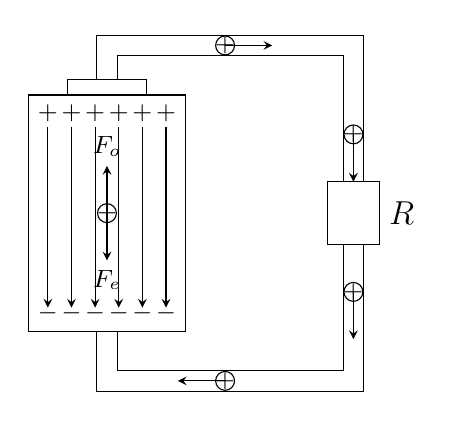
\begin{tikzpicture}
    \draw (-1,-1.5) rectangle (1,1.5); 
    \draw (-0.5,1.5) rectangle (0.5,1.7);
    \foreach \x in {-0.75,-0.45,-0.15,0.15,0.45,0.75}
    \draw (\x,1.5) node [anchor=north] {\small $+$};
    \foreach \x in {-0.75,-0.45,-0.15,0.15,0.45,0.75}
    \draw (\x,-1.5) node [anchor=south] {\small $-$};
    \foreach \x in {-0.75,-0.45,-0.15,0.15,0.45,0.75}
    \draw[<-,>=stealth] (\x,-1.2)--(\x,1.1);
    \draw (0,0) circle [radius=0.12] node {\small $+$};
    \draw[->,>=stealth] (0,0)--++(0,0.6) node [anchor=south] {\small $F_o$};
    \draw[->,>=stealth] (0,0)--++(0,-0.6) node [anchor=north] {\small $F_e$};
    \draw (0.13,1.7)--(0.13,2.0)--(3,2.0)--(3,0.4);
    \draw (-0.13,1.7)--(-0.13,2.26)--(3.26,2.26)--(3.26,0.4);
    \draw (0.13,-1.5)--(0.13,-2.0)--(3,-2.0)--(3,-0.4);
    \draw (-0.13,-1.5)--(-0.13,-2.26)--(3.26,-2.26)--(3.26,-0.4);
    \draw (2.8,-0.4) rectangle (3.46,0.4);
    \draw (3.46,0) node [anchor=west]{\large $R$};
    \draw (1.5,2.13) circle [radius=0.12] node {\small $+$};
    \draw[->,>=stealth] (1.5,2.13)--++(0.6,0);
    \draw (3.13,1) circle [radius=0.12] node {\small $+$};
    \draw[->,>=stealth] (3.13,1)--++(0,-0.6);
    \draw (3.13,-1) circle [radius=0.12] node {\small $+$};
    \draw[->,>=stealth] (3.13,-1)--++(0,-0.6);
    \draw (1.5,-2.13) circle [radius=0.12] node {\small $+$};
    \draw[->,>=stealth] (1.5,-2.13)--++(-0.6,0);
  \end{tikzpicture}
  \caption{电动势}
  \label{fig:diandongshi}
\end{figure}

在电源内部,正电荷所受电场力$F_e$ 方向由正极指向负极,但是电荷要完成闭合回路,所以必然存在非静电力$F_o$ 作用在电荷上,将它由正极移动到负极.显然非静电力$F_o$ 做正功,静电力$F_e$ 做负功,所以其它形式的能减少,电能增加,电源完成了将其它形式的能转化为电能的任务.不同的电源转化其它形式的能为电能的能力可以由转移单位电荷量,非静电力做的功来衡量,这个量称为电动势.所以电动势的定义为
\begin{equation}
  E=\frac{W_o}{q}
  \label{eq:diandongshi}
\end{equation}
式中$W_o$ 指非静电力做功,下角标$o$ 指 other 的意思.

\section{电场力做功}

在电路中电场力做功可以用电流和电压表达出来,它和微观电场中的情况相比形式上不太一样.同时,在后面的运算中经常需要处理能量和做功的问题,所以这里单独推导一下.

\begin{figure}[H]
  \centering
  \begin{tikzpicture}
    \draw (-3,-0.5) rectangle (3,0.5); 
    \draw[dashed] (-2,-0.7)--(-2,0.7);
    \draw[dashed] (2,-0.7)--(2,0.7);
    \filldraw (-2.5,-0.5) rectangle (-2,0.5);
    \filldraw (1.5,-0.5) rectangle (2,0.5);
    \draw[pattern =north west lines] (-2,-0.5) rectangle (-1.5,0.5); 
    \draw[pattern =north west lines] (2,-0.5) rectangle (2.5,0.5); 
    \draw (-2.25,0.5) node [anchor=south] {\small $A$};
    \draw (-1.75,0.5) node [anchor=south] {\small $B$};
    \draw (1.75,0.5) node [anchor=south] {\small $C$};
    \draw (2.25,0.5) node [anchor=south] {\small $D$};
    \draw[->,>=stealth] (-2.25,-0.5)--(-2.25,-1)--(-1.75,-1)--(-1.75,-0.5);
    \draw[->,>=stealth] (1.75,-0.5)--(1.75,-1)--(2.25,-1)--(2.25,-0.5);
    \draw[->,>=stealth,dashed](-2.25,0.5)--(-2.25,1.3)--(2.25,1.3)--(2.25,0.5);
    \draw[->,>=stealth] (-2,0)--++(0.8,0);
    \draw[->,>=stealth] (2,0)--++(0.8,0);
    \draw (-2,-0.6) node [anchor=north]{\small $\alpha$};
    \draw (2,-0.6) node [anchor=north]{\small $\beta$};
  \end{tikzpicture}
  \caption{电流做功的计算}
  \label{fig:dianluwork}
\end{figure}

如图\ref{fig:dianluwork}所示是一段导线,其中通有恒定电流,方向向右.经过一段时间$\Delta t$ ,这里发生的实际情况是$A$部分的电荷转移到了$B$, 同时$C$部分的电荷转移到了$D$,由于是恒定电流,所以电路中的电荷分布不会发生变化,结合电荷守恒定律可得$B$ 部分的电荷数量同$C$部分的电荷数量相同,所以$\alpha$ 到$\beta$ 一段的电荷数量是保持不变的.这在宏观看来就像是$A$部分的电荷通过$\alpha$面到$\beta$面直接转移到了$D$,于是电场力做的功就等于将电荷量$I\Delta t$从$A$移动到$D$电场力做的功,记$\alpha$和$\beta$ 间的电压为$U$,电流大小为$I$,则电场力做的功为
\begin{gather}
  W=I\Delta t \cdot \varphi_\alpha- I\Delta t \cdot \varphi_\beta=UI\Delta t
  \intertext{对应的电功率为}
  P=UI
\end{gather}


\section{焦耳定律}

焦耳定律是一条实验定律,它的形式可以由纯电阻电路推导出来.当电流通过一个纯电阻时,导体将会发热,这个热量记为$Q$,则由于是纯电阻,所以电能完全转化为热,同时电流和电压还满足欧姆定律,则
\begin{gather}
 \left\{
   \begin{gathered}
     Q=UIt\\
     U=IR
   \end{gathered}
 \right.
 \intertext{解得}
 Q=I^2Rt
\end{gather}
由于焦耳定律是实验定律,所以任何情况下计算电流通过导体的热量都使用它来计算,这里只是借助于能量转化与守恒定律及欧姆定律推导出这个表达式而己.

\section{路端电压和电动势的关系}

从能量转化与守恒定律的角度讲,非静电力做的功有两个去向,一个是电源内部克服阻力做功所产生的焦耳热,一个是整个外电路所消耗的电能.记电源电动势为$E$,路端电压$U$,电源的内阻为$r$,于是可以列出能量转化和守恒定律
\begin{gather}
  EI=UI+I^2r
  \intertext{约去电流$I$,得}
  E=U+Ir
  \intertext{上式有时也写作}
   U=E-Ir
\end{gather}

\section{闭合电路的欧姆定律}

\subsection{闭合电路的欧姆定律}

在上一节讨论了路端电压与电动势的关系,当外电路是\CJKunderwave{纯电阻}时,外电路的电流和电压符合欧姆定律,所以
\begin{gather}
  \left\{
    \begin{gathered}
      E=U+Ir\\
      U=IR
    \end{gathered}
  \right.
  \intertext{二式联立,消去电压$U$,解得}
  I=\frac{E}{R+r}
\end{gather}
上面的式子就是闭合电路的欧姆定律,鉴于这个公式描述的是整个电路的电动势、电流和电阻的关系,\CJKunderwave{原来的欧姆定律}从今以后称为\CJKunderwave{部分电路的欧姆定律}.

\subsection{纯电阻电路最大输出功率}

这一小节讨论一个闭合电路欧姆定律的重要应用---纯电阻电路的最大输出功率.当外电路为纯电阻时,记其阻值为$R$,电源的电动势为$E$,电源内阻为$r$,则输出功率为
\begin{gather}
  P=I^2R
  \intertext{其中电流可以由闭合电路的欧姆定律表达出来,从而将输出功率化为外电阻的函数}
  P=\left(\frac{E}{R+r}\right)^2R=\frac{E^2}{R+\frac{r^2}{R}+2r}
  \intertext{由均值不等式可求得其最大值,计算如下}
  P=\frac{E^2}{R+\frac{r^2}{R}+2r}\leqslant \frac{E^2}{2\sqrt{R\cdot\frac{r^2}{R}}+2r}=\frac{E^2}{4r}
  \intertext{上式当且仅当$R=\frac{r^2}{R}$时取等,即最大输出功率和条件分别为}
  P_{max}=\frac{E^2}{4r} \qquad R=r
\end{gather}
\section{串联和并联}
串是一种结构,联是一块同时工作的意思,所以串联是以串这种结构同时工作的意思.同理,并联是以并这种结构同时工作的意思.下面讨论纯电阻电路串联和并联的特点.
\subsection{串联电路}
如图\ref{fig:chuanlian}所示是串联结构,它是各个元件首尾相连构成.
\begin{figure}[H]
  \centering
  \begin{circuitikz}
    \draw (-3,0) to [R=$R_1$] (-1,0) to [R=$R_2$] (2,0);
    \draw[dashed] (2,0)--(3,0);
    \draw (3,0) to [R=$R_n$] (5,0);
    \draw (-3,0) node [anchor=south] {$\varphi_0$};
    \draw (-1,0) node [anchor=south] {$\varphi_1$};
    \draw (5,0) node [anchor=south] {$\varphi_n$};
    \draw[dashed] (-2.8,-1) rectangle (4.8,1);
  \end{circuitikz}
  \caption{串联电路}
  \label{fig:chuanlian}
\end{figure}

\subsubsection{串联电路的电流}

通过电阻$R_i$ 的电流记为 $I_i$ ,由于电荷守恒则相同时间内通过横截面的电荷量相都同,所以可以判断出来各电流是相等的.如图\ref{fig:chuanlian} 中方框内部可以看成一个整体,这个整体叫做等效电阻,通过它的电流记作 $I$ ,各部分电流的关系为
\begin{gather}
  I=I_1=I_2=I_3=\cdots=I_n
  \label{eq:chuanlianI}
\end{gather}

\subsubsection{串联电路的电压}

等效电阻两端的电压记作$U$,第$i$个电阻 $R_i$ 两端的电压记作 $U_i$.由电势差的定义可以得到
\begin{gather}
  \varphi_0-\varphi_n =(\varphi_0-\varphi_1)+(\varphi_1-\varphi_2)+\cdots +(\varphi_{n-1}-\varphi_n)
  \intertext{用电压写出以上关系就是串联电路各部分的电压关系}
  U=U_1+U_2+\cdots +U_n
  \label{eq:chuanlianU}
\end{gather}

\subsubsection{串联电路的等效电阻}

由串联电路的电压关系\eqref{eq:chuanlianU}左右同时除以电流$I$得
\begin{gather}
  \frac{U}{I}=\frac{U_1}{I}+\frac{U_2}{I} \cdots +\frac{U_n}{I}
  \intertext{由于电流关系\eqref{eq:chuanlianI}可以将上式写为}
  \frac{U}{I}=\frac{U_1}{I_1}+\frac{U_2}{I_2} \cdots +\frac{U_n}{I_n}
  \intertext{由欧姆定律可得等效电阻为}
  R=R_1+R_2+\cdots+R_n
\end{gather}

\subsubsection{拓展:串联电容器的电容}

如图\ref{fig:chuanlianC}所示,电容器$C_1$ 两个极板上的电荷量是相同的,但是由于 $C_1$和$C_2$ 是串联的,所以$C_1$的右板和 $C_2$的左板通过导线相连接,这两个板与外部电路是隔离开的,所以它是电中性的,则这两个板上的电荷量大小是相同的,但是电性相反,按此规律一直分析到最右边的一个电容器$C_n$ 则可以得到结论$C_1$的左板与$C_n$ 的右板带等量异种电荷.也就是说,这两个极板相当于构成一个电容器,也就是等效电容器.

\begin{figure}[H]
  \centering
  \begin{circuitikz}
    \draw (-3,0) to [C=$C_1$] (-1,0) to [C=$C_2$] (2,0);
    \draw[dashed] (2,0)--(3,0);
    \draw (3,0) to [C=$C_n$] (5,0);
    \draw (-3,0) node [anchor=south] {$\varphi_0$};
    \draw (-1,0) node [anchor=south] {$\varphi_1$};
    \draw (5,0) node [anchor=south] {$\varphi_n$};
    \draw[dashed] (-2.8,-1) rectangle (4.8,1);
  \end{circuitikz}
  \caption{串联电容器}
  \label{fig:chuanlianC}
\end{figure}

由前述分析可得各电容器在串联时带电量是相同的,所以
\begin{gather}
  Q=Q_1=Q_2=\cdots =Q_n
  \intertext{由串联电路的电压关系可得}
  U=U_1+U_2+\cdots +U_n
  \intertext{考虑到电容的定义可得}
  \frac{Q}{C}=\frac{Q_1}{C_1}+\frac{Q_2}{C_2}+\cdots +\frac{Q_n}{C_n}
  \intertext{分子上的电量由于都相同,所以可以消去,得等效电容为}
  \frac{1}{C}=\frac{1}{C_1}+\frac{1}{C_2}+\cdots +\frac{1}{C_n}
  \intertext{当两个电容串联时等效电容最容易写出,为}
  C=\frac{C_1C_2}{C_1+C_2}
\end{gather}

\subsection{并联电路}

如图\ref{fig:binglian}所示是并联电路的结构,各个元件的两端分别对应相连.

\begin{figure}[H]
  \centering
  \begin{circuitikz}
    \draw (-2,3) to [R=$R_1$] (2,3);
    \draw (-2,2) to [R=$R_2$] (2,2);
    \draw (0,1) node {$\cdots$};
    \draw (-2,0) to [R=$R_n$] (2,0);
    \draw (-2,0)--(-2,3);
    \draw (2,0)--(2,3);
    \draw (-3,1.5)--(-2,1.5);
    \draw (3,1.5)--(2,1.5);
    \draw[dashed] (-2.5,-0.8) rectangle (2.5,3.8);
  \end{circuitikz}
  \caption{并联电路}
  \label{fig:binglian}
\end{figure}

\subsubsection{并联电路的电流}

同样由电荷守恒定律可得,相同时间内干路中通过横截面的电量应当与各支路通过支路横截面的电量的和是相同的.所以得干路电流$I$ 等于各支路电流 $I_i$ 之和,即
\begin{gather}
 I=I_1+I_2+I_3+\cdots +I_n 
 \label{eq:binglianI}
\end{gather}

\subsubsection{并联电路的电压}

由电势差的定义可得各电阻两端的电势对应相等,所以它们的电压是相同的.记虚线框内部分为一个整体,则其两端的电压为$U$,各电阻$R_i$ 两端对应电压记为 $U_i$,即
\begin{gather}
  U=U_1=U_2=U_3=\cdots=U_n
 \label{eq:binglianU}
\end{gather}

\subsubsection{并联电路的等效电阻}

由并联电路电流关系\eqref{eq:binglianI}两端同时除以等效电压$U$,可得
\begin{gather}
  \frac{I}{U}=\frac{I_1}{U}+\frac{I_2}{U}+\cdots+\frac{I_n}{U}
  \intertext{由并联电路电压关系\eqref{eq:binglianU}可得,上式右侧中的电压可以对应加上下标,因为它们都相等,即}
  \frac{I}{U}=\frac{I_1}{U_1}+\frac{I_2}{U_2}+\cdots+\frac{I_n}{U_n}
  \intertext{由部分电路的欧姆定律可得}
  \frac{1}{R}=\frac{1}{R_1}+\frac{1}{R_2}+\cdots+\frac{1}{R_n}
  \intertext{上式存在一个特例,即当两个电阻并联时}
  R=\frac{R_1R_2}{R_1+R_2}
\end{gather}

\subsubsection{拓展:并联电容器的电容}

如图\ref{fig:binglianC}所示为电容器的并联,由于各电容器的极板的并联连接方式,则它们等效于一个大的电容器,此电容器的极板面积等于各电容器极板面积之和,再结合电荷守恒定律可得等效电容器的电容所带电荷量是各电容器所带电荷量之和.而且对于并联,则每一个电容器两端的电压是相同的,由这些条件就可以建立每个电容器的电容和等效电容的关系.

\begin{figure}[H]
  \centering
  \begin{circuitikz}
    \draw (-2,3) to [C=$C_1$] (2,3);
    \draw (-2,1.5) to [C=$C_2$] (2,1.5);
    \draw (0,1) node {$\cdots$};
    \draw (-2,0) to [C=$C_n$] (2,0);
    \draw (-2,0)--(-2,3);
    \draw (2,0)--(2,3);
    \draw (-3,1.5)--(-2,1.5);
    \draw (3,1.5)--(2,1.5);
    \draw[dashed] (-2.5,-0.8) rectangle (2.5,4);
  \end{circuitikz}
  \caption{并联电容器的电容}
  \label{fig:binglianC}
\end{figure}

由前述可知,等效电容的电荷量等于各电容器电量之和,即
\begin{gather}
  Q=Q_1+Q_2+\cdots+Q_n
  \intertext{再考虑电容的定义可得}
  CU=C_1U_1+C_2U_2+\cdots +C_nU_n
  \intertext{由于并联时电压都相等,所以可以将上式中的电压约掉,则得到等效电容是各部分电容之和的结论,即}
  C=C_1+C_2+\cdots +C_n
\end{gather}


\section{电阻定律}

如图\ref{fig:dianzulaw}所示一段金属导体,为了方便讨论我们把它的横截面画为矩形,其它对于其它的形状只要我们取的矩形足够小,则也可以实现这里的代替.\footnote{比如求圆的面积时,我们也可以采用微元法将其分割成无限多个小矩形,然后再相加便得到圆的面积.}

\begin{figure}[H]
  \centering
  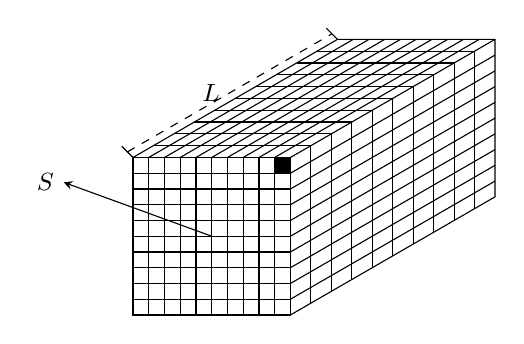
\begin{tikzpicture}
    \draw (-1,-1) rectangle (1,1); 
    \foreach \x in {-0.8,-0.6,-0.4,-0.2,0,0.2,0.4,0.6,0.8}
    \draw (\x,-1)--(\x,1);
    \foreach \x in {-0.8,-0.6,-0.4,-0.2,0,0.2,0.4,0.6,0.8}
    \draw (-1,\x)--(1,\x);
    \draw (1,-1)--++(30:3)--++(0,2)--++(-2,0);
    \draw (1,1)--++(30:3);
    \draw (-1,1)--++(30:3);
    \foreach \x in {-0.8,-0.6,-0.4,-0.2,0,0.2,0.4,0.6,0.8}
    \draw (1,\x)--++(30:3);
    \foreach \x in {-0.8,-0.6,-0.4,-0.2,0,0.2,0.4,0.6,0.8}
    \draw (\x,1)--++(30:3);
    \foreach \x in {0.3,0.6,0.9,1.2,1.5,1.8,2.1,2.4,2.7}
    \draw (1,-1)++(30:\x)--++(0,2)--++(-2,0);
    \filldraw (1,1) rectangle (0.8,0.8);
    \draw(-1,1)--++(135:0.2);
    \draw(-1,1)++(30:3)--++(135:0.2);
    \draw[dashed] (-1,1)++(135:0.1)--++(30:3);
    \draw (-1,1)++(135:0.1)++(30:1.5) node [anchor=east]{\small $L$};
    \draw[->,>=stealth] (0,0)--++(160:2) node [anchor=east] {\small $S$};
  \end{tikzpicture}
  \qquad
  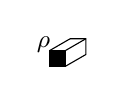
\begin{tikzpicture}
    \filldraw (0,0) rectangle (0.2,0.2); 
    \draw (0.2,0)--++(30:0.3)--++(0,0.2)--++(-0.2,0);
    \draw (0.2,0.2)--++(30:0.3);
    \draw (0,0.2)--++(30:0.3);
    \draw (0,0.2)++(30:0.15) node [anchor=east]{\small $\rho$};
  \end{tikzpicture}
  \caption{电阻定律}
  \label{fig:dianzulaw}
\end{figure}

图\ref{fig:dianzulaw} 中所画导体的横截面积为$S$,导体的长度为$L$,我们在思想上做了如图所示的分割,即将面积划分为$S$个面积为$1$ 的部分,同时将长度也划分为长度为$l$的部分,这样划分之后我们便得到$S\times L$ 个右图所示的小部分.将这个单位体积,接入电路中时其电阻为$\rho$,这个$\rho$叫做电阻率(单位是$\Omega \cdot m$),它是单位体积单位面积单位长度的这个部分的阻值,所以同种材料的电阻率是相同的,但是不同材料的电阻率就是不同的.因此,电阻率可以作为区别不同导体导电性能的物理量.

我们由电阻率可以求出电阻的大小,首先我们将$L$个单元串联起来,则这一条的阻值为
\begin{gather}
  \rho \cdot L
  \intertext{这样的条一共有$S$ 个,我们再将这$S$ 条导体并联起来,则等效阻值为$R$,在这里就是真正的电阻}
  \frac{1}{R}=\frac{1}{\rho L}+\frac{1}{\rho L}+\cdots +\frac{1}{\rho L}
  \intertext{右式中共有$S$个相同的项相加,计算可得}
  R=\rho\frac{L}{S}
\end{gather}
上式就是著名的电阻定律.对于横截面不同的导体我们总是可以划分的足够细致而得到上面相同的结论,比如横截面为圆的时候,同学们可以自行讨论.
